\chapter{Anatomía Animal comparada}
\section{Elementos de morfología}
\subsection{Simetría}
\paragraph{Morfología}: Ciencia auxiliar cuyo objeto es el estudio son los animales desde el punto de vista geométrico.
\paragraph{Ejes}: Línea imaginaria que atraviesa al animal de forma que todos sus elementos se encuentran en torno a ella. Se pueden diferenciar:
\begin{itemize}[itemsep=0pt,parsep=0pt,topsep=0pt,partopsep=0pt]
    \item \textbf{Eje oral-aborall}: desde la boca hasta el ano.
    \item\textbf{Eje apical-antiapical}: desde el extremo superior al inferior
\end{itemize}
\paragraph{Plano}: plano que corta al animal en dos imágenes especulares:
\begin{itemize}[itemsep=0pt,parsep=0pt,topsep=0pt,partopsep=0pt]
    \item \textbf{Sagital}: divide al animal en una parte izquierda y otra derecha.
    \item\textbf{Frontal}: divide al animal en una parte dorsal y otra ventral.
    \item\textbf{Transversal}: divide al animal en una parte anterior y otra posterior.
\end{itemize}
\begin{figure}[H]
    \centering
    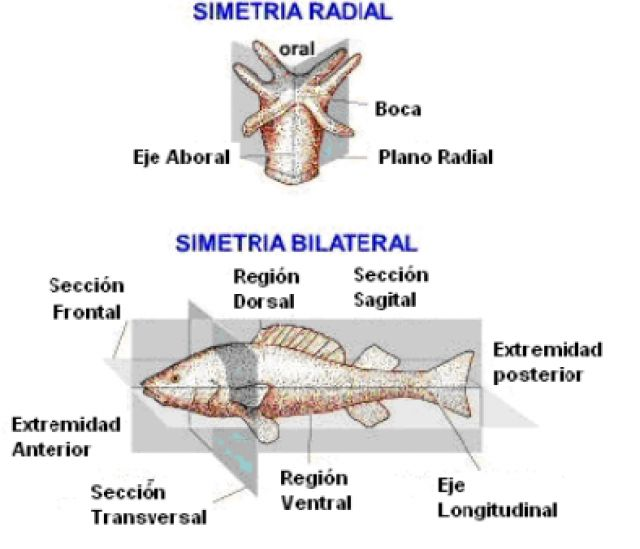
\includegraphics[width=0.65\columnwidth]{A.imagenes/ACV-ANATANIM-EjesPlanos}
    \caption[Ejemplos de Ejes y planos de simetría]{Ejemplos de Ejes y planos de simetría, en animales de simetría radial y de simetría bilateral.}
\end{figure}
\subsection{Clasificación morfológica}
\begin{itemize}[itemsep=0pt,parsep=0pt,topsep=0pt,partopsep=0pt]
    \item \textbf{Anoxonía}: No tienen ejes ni planos de simetría. Son organismos simples (amebas o poríferos), sésiles y poco evolucionados. Los individuos de la misma especie no son siempre iguales.
    \item\textbf{Homoaxonía}: son múltiples (infinitos) ejes homopolares e infinitos planos. Son organismos no animales (radiolarios, protozoos), esféricos.
    \item\textbf{Monoaxonía}: gran mayoría de animales, solo poseer un eje de simetría. Se dividen según planos en:
    \begin{itemize}[itemsep=0pt,parsep=0pt,topsep=0pt,partopsep=0pt]
        \item \textbf{Simetría radial}: infinitos planos de simetría un único eje. Son organismos simples, sésiles o poco móviles, habitan en el fondo marino.
        \item\textbf{Simetría birradial}: un eje de simetría y dos planos simétricos. Son organismos simples, śesiles o poco móviles, como los \textit{Cnidaria},$\dots$
        \item\textbf{Simetría pentaradial}: un eje de simetría y cinco planos de simetría (las partes del animal se repiten cinco veces. Propio de los equinodermos.
        \item\textbf{Simetría bilateral}: lo tienen gran cantidad de animales. Tienen una cabez (contiene centros nerviosos y se encuentran órganos de los sentidos). Son organismos complejos y con plano de simetría sagital. Determina la dirección del desplazamiento. Se distinguen dos regiones, por la cefalización:
        \begin{itemize}[itemsep=0pt,parsep=0pt,topsep=0pt,partopsep=0pt]
            \item \textbf{Cefálica}: contiene la zona oral y la cabeza y es la parte anterior.
            \item\textbf{Caudal}: contiene el resto del organismo del animal no incluida en la zona cefálica. Es la parte posterior.
        \end{itemize}
    \end{itemize}
    \item\textbf{Asimetrías}: alteraciones a la simetría:
    \begin{itemize}[itemsep=0pt,parsep=0pt,topsep=0pt,partopsep=0pt]
        \item \textbf{Organización interna}: el animal tiene órganos impares, diferenciandose dos partes desiguales internas.
        \item\textbf{Por uso}: el animal da preferencia al uso de una parte de su cuerpo en detrimento de su homóloga en la otra sección para una determinada acción (como zurdo$\leftrightarrows$diestro). Deriva de una laterización.
        \item\textbf{Ofensivo-Defensivo}: Una parte se ve más desarrollada que su homóloga, sirviendo al animal, para atacar o defenderse (por ejemplo, el cangrejo violinista).
        \item\textbf{Prefijado}: el animal hipertrofia una parte de su cuerpo (Narval, que desarrolla un colmillo para compensar a otro).
        \item\textbf{Por desarrollo}: el animal cambia o desarrolla una asimetría que se completa en la edad adulta (ej. osteictios pleuronectiformes).
        \item\textbf{Dobles simetrías}: animales segmentados.
        \item\textbf{Clinasimetría}: en un hemisferio y en otro tiene diferentes simetrías (ej. cnidarios en colonias, como el género \textit{Velella}).
    \end{itemize}
\end{itemize}
\subsection{Estructuras morfológicas}
\paragraph{Proglótides}: propia de los platelmintos (Cestodos). Se trata de un órgano sexual, sección de un estróbilo y no imprescindible. Es hermafrodita. Aumenta su grado de maduración con el alejamiento del escolex. Tienen tres fases:
\begin{enumerate}[itemsep=0pt,parsep=0pt,topsep=0pt,partopsep=0pt]
    \item Órgano sexual masculino.
    \item Órgano sexual femenino.
    \item Huevos (ruptura del proglótide y salen al exterior).
\end{enumerate}
\paragraph{Metámeros}: se da en los anélidos. El cuerpo se encuentra segmentado en anillos, imprescindibles (no se segmentan) y no regenerables. Cada sección contiene un vaso sanguineo dorsal y otro ventral, metanefridios (parte excretor, en la parte ventral), un cordón nervioso y una sección del tubo digestivo.
\begin{figure}[H]
    \centering
    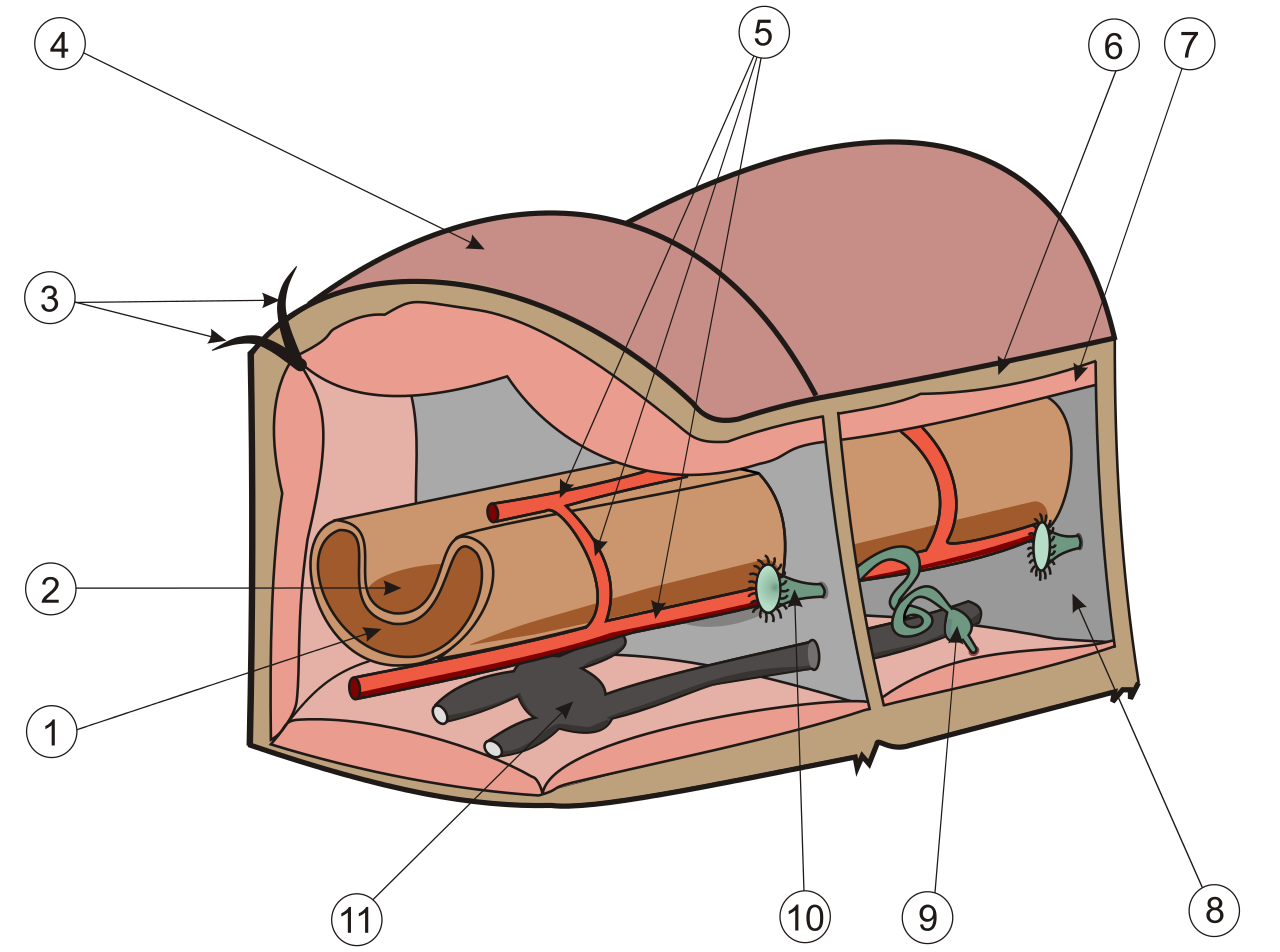
\includegraphics[width=0.5\columnwidth]{A.imagenes/ACV-ANATANIM-Metameros}
    \caption[Anatomía de un metámero]{Anatomía de un metámero: 1 - Lumen intestinal, 2 - Tiflosolio, 3 - Quetas, 4 - Cutícula, 5 - Vasos sanguíneos, 6 - Epitelio, 7 - Musculatura circular, 8 - Tabique del metámero, 9 - Célula terminal del metanefridio, conectando con el canal del metanefridio, 10 - Metanefridio, 11 - Ganglio nervioso del metámero.}
\end{figure}
\paragraph{Ciclómero}: propio de equinodermos y animales con simetría radial. Parte repetida circularmente, con los mismos órganos y estructuras (pueden regenerarse). Animales no cefalizados, cada brazo o sección tiene un tubo digestivo independiente, unas gónadas, un fotorreceptor y un sistema nervioso.
\paragraph{Tagma}: característico de artrópodos. Se da la unión de partes dedicadas a una misma función. Cada parte es la unión de metámeros dedicados a realizar una función, formando una unidad superior.  Se pueden distinguir un tagma cefálico (prostomeo y parte de un metámero), tagma torácico (función de movimiento de los metámeros y tubo digestivo), y tagma abdominal (reproducción).
\subsection{Clasificación del tipo de vida}
\begin{itemize}[itemsep=0pt,parsep=0pt,topsep=0pt,partopsep=0pt]
    \item Según su tipo de vida:
    \begin{itemize}[itemsep=0pt,parsep=0pt,topsep=0pt,partopsep=0pt]
        \item \textbf{Vida libre}: no viven pegados a otro ser.
        \item\textbf{Parásito}: vive fijado a un huésped. Si es en el exterior, se denomina ectoparásito; si está en el interior del ser vivo, es un endoparásito.
    \end{itemize}
    \item Según el medio que habitan:
    \begin{itemize}[itemsep=0pt,parsep=0pt,topsep=0pt,partopsep=0pt]
        \item \textbf{Terrestres}: viven sobre la superficie terrestre. Pueden ser epígeos (viven sobre la capa del suelo) o hipógeos (viven enterrados en la capa del suelo).
        \item\textbf{Acuáticos}: viven en la hidrosfera. Son dulceauicolas (viven en medios fluviales) o marinos (viven en el mar).
    \end{itemize}
    \item Seres acuáticos:
    \begin{itemize}[itemsep=0pt,parsep=0pt,topsep=0pt,partopsep=0pt]
        \item \textbf{Holobiontes}: el animal vive siempre en el mismo medio. Pueden ser talasobiontes (viven en el mar) o potamobiontes (viven en rios).
        \item\textbf{Anfiobiontes}: el animal vive una parte de su desarrollo en el mar o en rio y otra en el medio contrario. Según donde desovan son talasotocos (lo hacen en el mar), o potamotocos (lo hacen en el río).
    \end{itemize}
    \item Seres marinos:
    \begin{itemize}[itemsep=0pt,parsep=0pt,topsep=0pt,partopsep=0pt]
        \item \textbf{Bentónicos}: viven en el lecho marino (sésiles o poco móviles)
        \item\textbf{Pelágicos}: viven entre el fonto y la superficie marina (organismos nadadores).
        \item\textbf{Planctónicos}: viven en la superficie marina (arrastrados por la corriente).
    \end{itemize}
    \item Seres según su movilidad:
    \begin{itemize}[itemsep=0pt,parsep=0pt,topsep=0pt,partopsep=0pt]
        \item\textbf{Móvil}: se mueven.
        \item\textbf{Sécil} : se fijan al sustrato.
    \end{itemize}
    \item En relación a los comportamientos sociales:
    \begin{itemize}[itemsep=0pt,parsep=0pt,topsep=0pt,partopsep=0pt]
        \item \textbf{Solitarios}: no dependen unas de otros, viven en colonias ni tienen división de funciones.
        \item\textbf{Gregarios}: se reúnen en grupos con división de funciones.
        \item\textbf{Coloniales}: viven juntos y comparten partes del cuerpo.
    \end{itemize}
\end{itemize}
\section{Clasificación sistemática}
Se denomina \textbf{Taxonomía} a la ciencia auxiliar que ordena a los seres vivos con unas características comunes. Así mismo, una especie es la única categoría real, conjunto de seres vivos que se pueden reproducir entre si y que su descendencia sea fértil.
\section{\textit{Phylum Chordata}}
Los cordados tienen como características principales:
\begin{itemize}[itemsep=0pt,parsep=0pt,topsep=0pt,partopsep=0pt]
    \item \textbf{Epineuros}: tienen un tubo neural dorsal.
    \item\textbf{Faringotremados}: en algún momento de su desarrollo tienen una faringe perforada.
    \item\textbf{Cordados}: en algún momento de su vida tiene un esqueleto que es un filamento denominado corda. Es el soporte del cuerpo y eje esquelético donde se enganchan los músculos.
    \item En algún momento de su vida desarrollan una cola detrás del ano sin vísceras.
\end{itemize}
\subsection{Subfilo \textit{Tunichata} o Urocordados}
Subiertos por una capa (túnica). Sufren una metamorfosis drástica: de una cría con aspecto de renacuajo y con las características propias de los cordados, pasan a un adulo sin corda, tubo neural y cola. Se diferencian tres clases:
\begin{itemize}[itemsep=0pt,parsep=0pt,topsep=0pt,partopsep=0pt]
    \item \textbf{Ascideos}: tiene tres comportamientos sociales: sésiles, bentónicos y planctónicos.
    \item\textbf{Taliaceos}: son transparentes y planctónicos.
    \item\textbf{Apendicularios}: conservan todos los caracteres de los cordados.
\end{itemize}
\subsection{Subfilo \textit{Cephalochordata}}
También llamados anfioxos, tiene dos ejes y forma de huso. La corda les llega hasta la cabeza.
\subsection{Subfilo \textit{Vertebrata}}
Tienen el tubo neural tapado por vértebras. Se diferencian dos grupos principales:
\begin{itemize}[itemsep=0pt,parsep=0pt,topsep=0pt,partopsep=0pt]
    \item \textbf{Aganatos}: no tienen mandíbula, son:
    \begin{itemize}[itemsep=0pt,parsep=0pt,topsep=0pt,partopsep=0pt]
        \item \textbf{\textit{Myxines}}: saprófitos, al comer se enganchan al trozo a engullir, se anuda sobre sí mismos y al sacar la cabeza arrancan el alimento.
        \item\textbf{Lampreas}: ectoparásitos hematófogos, en la boca tienen una ventosa dentada, al igual que su lengua. Se agarra al huésped con la ventosa y este es perforado con la lengua.
    \end{itemize}
    \item\textbf{Gnatostomados}: tienen mandíbulas:
    \begin{itemize}[itemsep=0pt,parsep=0pt,topsep=0pt,partopsep=0pt]
        \item \textbf{Condríctios}: animales acuáticos, con branquias y esqueleto cartilaginoso. Anamniotas. Algunos representantes son las rayas o el tiburón.Se dividen en:
        \begin{itemize}[itemsep=0pt,parsep=0pt,topsep=0pt,partopsep=0pt]
            \item \textbf{Holocéfalos}: tienen un único agujero branquial. Se llaman, por su forma, \textit{quimeras monstruosas}.
            \item\textbf{Elasmobránquios}: tienen más de dos hendiduras branquiales.
        \end{itemize}
        \item\textbf{Osteíctios}: animales acuáticos con esqueleto óseo.Anamniotas. Se diferencian:
        \begin{itemize}[itemsep=0pt,parsep=0pt,topsep=0pt,partopsep=0pt]
            \item \textbf{Actinopterigios}: sólo tienen branquias.
            \item\textbf{Sarcopterígios}: tiene estructuras que darán lugar a pulmones.
        \end{itemize}
        \item\textbf{Anfibios}: animales de vida terrestre en hábitats húmedos.Anamniotas, de respiración pulmonar y cutánea. Necesitan un medio acuático o húmedo para reproducirse: los huevos se secarían. Las crias respiran bajo el agua.Se clasifican:
        \begin{itemize}[itemsep=0pt,parsep=0pt,topsep=0pt,partopsep=0pt]
            \item \textbf{Anuros}: sin cola.
            \item\textit{Urodelos}: con cola postanal sin vísceras.
        \end{itemize}
        \item\textbf{Reptiles}: animales de vida terrestre, amniotas y de respiración pulmonar. Se dividen según los agujeros craneales:
        \begin{itemize}[itemsep=0pt,parsep=0pt,topsep=0pt,partopsep=0pt]
            \item \textbf{Anápsidos}: no tienen agujeros craneales. (tortugas)
            \item\textbf{Diápsidos}: tienen dos agujeros en el cráneo , animales modernos . (serpientes).
            \item\textbf{Arcosaurios}: tienen dos agujeros en el cráneo, animales antiguos. (cocodrilos).
        \end{itemize}
        \item\textbf{Aves}: animales de vida terrestre, amniotas de respiración pulmonar. Tienen un cráneo derivado de un diápsido. Se pueden establecer:
        \begin{itemize}[itemsep=0pt,parsep=0pt,topsep=0pt,partopsep=0pt]
            \item \textbf{Ratites}: aves corredoras, no buceadoras ni voladoras, como el kiwi.
            \item\textbf{Impennes}: aves buceadoras, no corredoras ni voladoras, como el pingüino.
            \item\textbf{Carenados}: aves voladoras o que tienen estructuras preparadas para el vuelo.
        \end{itemize}
        \item\textbf{Mamíferos}: animales de vida terrestre, amniotas y de respiración pulmonar.
        \begin{itemize}[itemsep=0pt,parsep=0pt,topsep=0pt,partopsep=0pt]
            \item \textbf{Prototerios}: ponen huevos (ornitorrincos).
            \item\textbf{Terios}: no ponen huevos.
            \begin{itemize}[itemsep=0pt,parsep=0pt,topsep=0pt,partopsep=0pt]
                \item \textbf{Metaterios}: las crías nacen sin terminar de desarrollar, por lo que migran a una bolsa o marsupio donde terminan su desarrollo.
                \item\textbf{Euterios}: paren crías desarrolladas pero no siempre independientes.
            \end{itemize}
        \end{itemize}
    \end{itemize}
\end{itemize}
\begin{figure}[H]
    \centering
    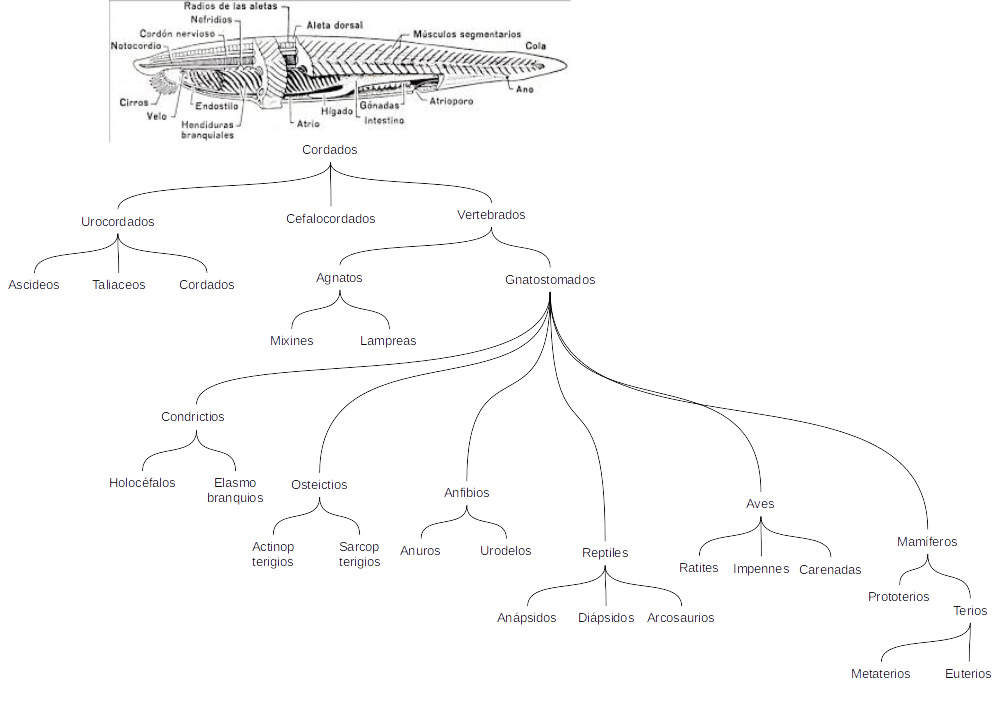
\includegraphics[width=\columnwidth]{A.imagenes/ACV-ANATANIM-Cordados}
    \caption{Clasificación y plan general de los cordados}
\end{figure}
\section{Desarrollo ontogenético}
Historia del desarrollo de un zigoto diplonte hasta que el individuo muere. Comprende:
\begin{itemize}[itemsep=0pt,parsep=0pt,topsep=0pt,partopsep=0pt]
    \item \textbf{Desarrollo embrionario}: observación de las distintas fases del zigoto. El desarrollo embrionario es algo exclusivo del reino \textit{Animalia}. Modos de reproducción:
    \begin{itemize}[itemsep=0pt,parsep=0pt,topsep=0pt,partopsep=0pt]
        \item \textbf{Reproducción asexual}: aquella en la que no hay meiosis, todos los individuos son clónicos.
        \item\textbf{Reproducción sexual}: aquella en la que hay meiosis. Es la única posible en los vertebrados. Se necesita un espermatozoide y un óvulo haploides formando un zigoto diploide. Puede ser mono o diparental, según intervengan uno o dos individuos.
    \end{itemize}
    \item\textbf{Desarrollo postembrionario}: paso del embrión al adulto y su posterior muerto.
\end{itemize}
\subsection{Zigoto: segmentación y gastrulación}
El zigoto es una célula resultante de la unión de dos gametos procedentes de dos gónadas distintas. Se distinguen por la distribución del vitelo, en cuatro tipos, que determinan la división celular.  Tras la formación del cigoto, llevará a cabo un proceso de segmentación, que es el conjunto de cariocinesis que lleva a cabo el zigoto para la formación de la gastrula. La gastrula es a su vez el proceso de invaginación del cigoto, formándose un blastoporo, orificio que comunica el exterior con el arquénteron (cavidad interna que dará lugar al endodermo).

Se pueden diferenciar cuatro tipos de zigoto:
\begin{itemize}[itemsep=0pt,parsep=0pt,topsep=0pt,partopsep=0pt]
    \item \textbf{Isolecito}: la materia nutritiva (vitelo) se reparte en pequeños gránulos uniformemente.
    \begin{itemize}[itemsep=0pt,parsep=0pt,topsep=0pt,partopsep=0pt]
        \item \textbf{Segmentación}: sufre una división igual y holoblástica (todos los blastómeros o células que forman la blástula, son iguales). El proceso consiste en sucesivos ciclos de mitosis iguales. En algunas especies, los blastómeros no son paralelos ni perpendiculares entre sí, si no que se desplazan uno respecto al otro, dando lugar a una diferenciación en segmentaciones radiales o espirales.
        \item\textbf{Gastrulación}: tanto las blástulas espirales como las radiales, las células de un polo sufren unas mitosis más acelaradas creando una región hueca, cuyo tapiz generará el endodermo, mientras que las células en el exterior dan lugar al ectodermo.
    \end{itemize}
    \item\textbf{Heterolocito}: el vitelo se reparte en gránulos pequeños en un polo animal y en gránulos grandes en polo vegetativo.
    \begin{itemize}[itemsep=0pt,parsep=0pt,topsep=0pt,partopsep=0pt]
        \item \textbf{Segmentación}: se dan dos subfases:
        \begin{itemize}[itemsep=0pt,parsep=0pt,topsep=0pt,partopsep=0pt]
            \item \textit{Hasta el cliclo segundo}: se tratan de divisiones holoblásticas e iguales resultando cuatro células (2 en el polo animal y dos en el polo vegetativo). Se diferencia así un polo vegetativo de crecimiento lento (por falta de vitelo) y un polo animal de crecimiento rápido.
            \item\textit{Hasta la blástula}: se da una división holoblástica desigual, pudiendo segmentarse radial o espiralmente. En cualquier caso, se crean dos tipos de células: micrómeros (blastómeros pequeños) y macrómeros (blastómeros grandes).
        \end{itemize}
        \item\textbf{Gastrulación}: En este caso, las células del endodermo son los macrómeros, de forma que el endodermo siempre lo forma el polo vegetativo.
    \end{itemize}
    \item\textbf{Telolecito}: vitelo gigante que rellena todo el cigote, dando un núcleo lateralizado.
    \begin{itemize}[itemsep=0pt,parsep=0pt,topsep=0pt,partopsep=0pt]
        \item \textbf{Segmetación}: Se dividen los nucleos en uno de los polos de la célula pero sin división citoplasmática. Tras un cierto número de ciclos, los núcleos forman protuberancias en la membrana, independizandose y generando un discoblasto. Los blastómeros irán consumiendo poco a poco el vitelo.
    \end{itemize}
    \item\textbf{Centrolecito}: vitelo gigante que rodea a un núcleo que se situa en el centro rodeado por vitelo.
    \begin{itemize}[itemsep=0pt,parsep=0pt,topsep=0pt,partopsep=0pt]
        \item \textbf{Segmetación}: En un primer paso, el nucleo migra a uno de los polos, dando lugar a un zigoto telolecito. Se dividen los nucleos en uno de los polos de la célula pero sin división citoplasmática. Tras un cierto número de ciclos, los núcleos forman protuberancias en la membrana, independizandose y generando un discoblasto. Los blastómeros irán consumiendo poco a poco el vitelo.
    \end{itemize}
\end{itemize}

El desarrollo embrionario puede continuar de dos formas:
\begin{itemize}[itemsep=0pt,parsep=0pt,topsep=0pt,partopsep=0pt]
    \item No se forma una tercera hoja embrionaria (animales diblásticos: Cnidarios y tenóferos). Estos animales desarrollan tejidos producidos por estas dos hojas: epidermis, sistema nervioso y tubo digestivo.
    \item Se forma una tercera hoja emprionaria (animales triblásticos). Apartir del endodermo, se forma una tercera hoja embrionaria o mesodermo. Se pueden diferenciar por dos procesos: esquizocelia y enterocelia. Según la formación del celoma, pueden ser: acelomados, pseudocelomados, celomados o enterocelomados.
\end{itemize}
\begin{figure}[H]
    \centering
    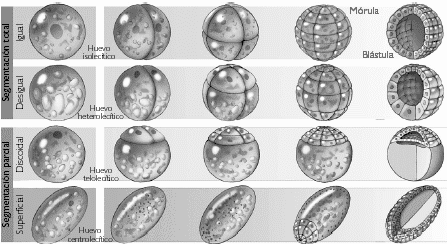
\includegraphics[width=0.8\columnwidth]{A.imagenes/ACV-ANATANIM-SegmetacionGastrulacion}
    \caption[Tipos de cigoto y modelos de segmentación]{Tipos de cigoto y modelos de segmentación. Primeras fases del desarrollo embrionario en los animales y tipos de segmentación según la cantidad y disposición del vitelo nutritivo.}
\end{figure}
\begin{figure}[H]
    \centering
    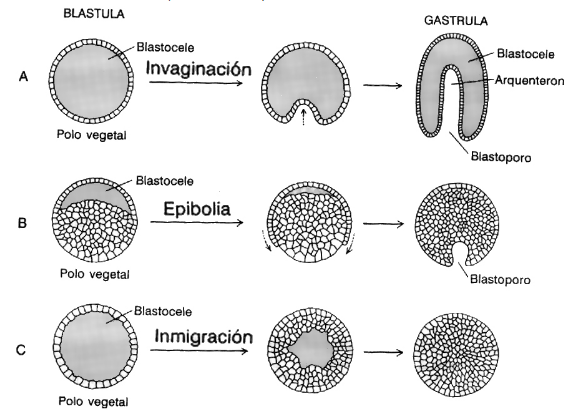
\includegraphics[width=0.7\columnwidth]{A.imagenes/ACV-ANATANIM-Gastrulacion}
    \caption[Modelos de gastrulación]{Modelos de gastrulación. A, por invaginación: las células del polo vegetal del embrión se invaginan y forman el arquénteron; la abertura al exterior es el blastoporo; B, por epibolia: las células del polo animal del embrión crecen para recubrir las del polo vegetal; en este caso el blastoporo se puede formar más tarde; C, por inmigración: las células de la pared interna de la blástula caen al interior del blastocele, formando una masa que luego se ahuecará para formar un arquénteron. Existen aún más modalidades. }
\end{figure}
\subsection{Hojas embrionarias}
Una hoja embrionaria es el conjunto de células formadoras durante el desarrollo embrionario a partir de las cuales se generarán los diversos órganos y tejidos.
\begin{itemize}[itemsep=0pt,parsep=0pt,topsep=0pt,partopsep=0pt]
    \item \textbf{Ectodermo}: 
    \begin{itemize}[itemsep=0pt,parsep=0pt,topsep=0pt,partopsep=0pt]
        \item Epidermis
        \item Sistema nervioso
        \item Boca, faringe, recto y ano.
    \end{itemize}
    \item \textbf{Endodermo}:
    \begin{itemize}[itemsep=0pt,parsep=0pt,topsep=0pt,partopsep=0pt]
        \item Tubo digestivo
        \item Glándulas anejas
        \item Células germinales
    \end{itemize}
    \item\textbf{Mesodermo}: 
    \begin{itemize}[itemsep=0pt,parsep=0pt,topsep=0pt,partopsep=0pt]
        \item Dermis
        \item Aparato circulatorio
        \item Musculatura y esqueleto (vertebrados)
        \item Aparato excretor
        \item Aparato reproductor (células no germinales)
        \item Aparato respiratorio (no faringe)
    \end{itemize}
\end{itemize}

Cada una de las estructuras se formará mediante organogénesis que es el proceso de formación del órgano a partir de las hojas embrionarias.
\subsection{Blastoporo}
El blastoporo (lugar que comunica el arquenteron con el exterior) diferencia a dos tipos de animales:
\begin{itemize}[itemsep=0pt,parsep=0pt,topsep=0pt,partopsep=0pt]
    \item \textbf{Protóstomos}: animales de segmentación espiral, del blastoporo permanece abierto y formará la boca.
    \item\textbf{Deuteróstomos}: animales de segmentación radial, el blastoporo se cierra y la boca es de neoformación.
\end{itemize}
\subsection{Formación del mesodermo}
El proceso de formación del mesodermo o embolia puede darse de dos formas:
\begin{itemize}[itemsep=0pt,parsep=0pt,topsep=0pt,partopsep=0pt]
    \item \textbf{Animales de segmentación espiral}: al ser animales con una determinación muy temprana, se puede localizar que blastómeros dan lugar al mesodermo. En este caso, es el blastómero 4D, sitá junto al blastoporo. Por un proceso de mitosis repetidas forma el mesodermo, siguiendo uno de estos tres procesos:
    \begin{itemize}[itemsep=0pt,parsep=0pt,topsep=0pt,partopsep=0pt]
        \item \textbf{Animales acelomados}: (platelmintos) todo el blastocele (cavidad interior de la blástula) se rellena de mesodermo y no forma celoma.
        \item\textbf{Animales pseudocelomados}: (nemátodos) el mesodermo se pega al ectodermo, formando una cavidad, el pseudoceloma.
        \item\textbf{Animales celomados}: (anélidos, moluscos y artrópodos) los blastómeros del mesodermo forman unas esferas huecas cuyo interior se denomina celoma. Este proceso es la esquizocelia y necesita la migración a través del blastocele hasta el ecuador.
    \end{itemize}
    \item\textbf{Animales de segmentación radial}: el mesodermo se forma por enterocelia, un proceso exclusivo de cordados y equinodermos. Al ser animales de diferenciación tardía, los blastómeros que forman el endodermoestán determinados por la posición. En la enterocelia, el mesodermo se forma a partir del endodermo: de este, y por rápidas mitosis, se forman unas invaginaciones que acaban independizándose y formando una vesículas huecas con el celoma en su interior. 
\end{itemize}
\begin{figure}[H]
    \centering
    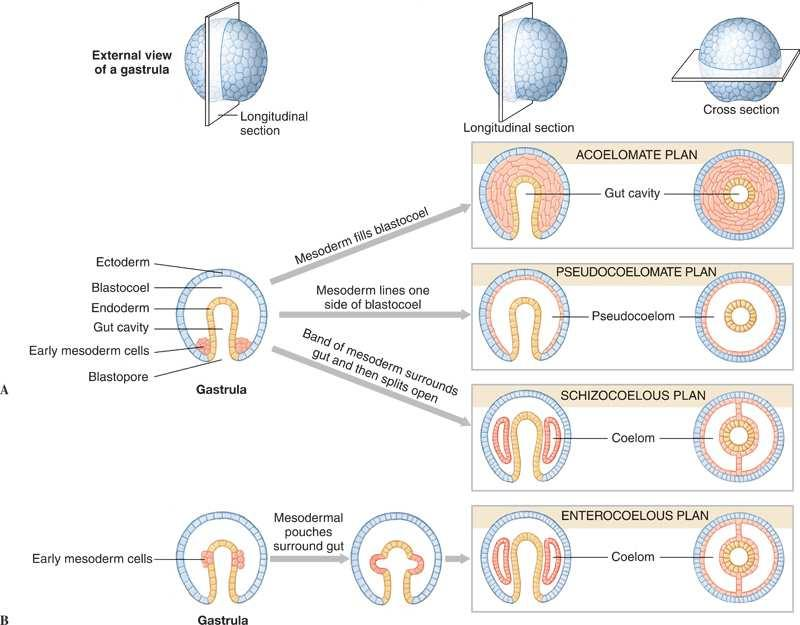
\includegraphics[width=\columnwidth]{A.imagenes/ACV-ANATANIM-Mesodermo.jpeg}    
    \caption[Modelos de formación del mesodermo]{Modelos de formación del mesodermo. A, modelos de formación del mesodermo en animales de segmentación espiral; B, modelos de enterocelia para animales de segmentación radial.}
\end{figure}
\subsection{Desarrollo postembrionario}
Se diferencian tres tipos de ciclo:
\begin{itemize}[itemsep=0pt,parsep=0pt,topsep=0pt,partopsep=0pt]
    \item \textbf{Ciclo directo}: animales con cigotos con gran cantidad de vitelo. Esto permite a la cría desarrollarse por completo, naciendo un juvenil de apariencia similar al adulto pero de menor tamaño.
    \item\textbf{Ciclo metagenético}: se da con o sin larva. La forman dos individuos adulots que conforman dos subfases del ciclo, en una hay reproducción sexual; y en la otra, reproducción asexual. Un ejemplo son los cnidarios.
    \item\textbf{Ciclo indirecto}: la larva difiere de la morfología del adulto, llegando a no reconocerse. Propio de zigotos con poco vitelo, se diferencian varias funciones a este ciclo vital como la dispersión (en los tunicados, el adulto sésil permite que la especie colonice nuevos territorios); la alimentación juvenil (la larva se alimenta para obtener los nutrientes para poder madurar); o evitar competencia con el adulto con respecto a recursos alimentarios y que no peligre la especie. Así mismo, se diferencian dos tipos de metamorfosis:
    \begin{itemize}[itemsep=0pt,parsep=0pt,topsep=0pt,partopsep=0pt]
        \item \textbf{Gradual} o \textbf{hemimetábula}: se forman nuevas estructuras de forma gradual (por ejemplo, anfibios anuros como la rana).
        \item\textbf{Dŕastica} o \textbf{Homometábula}: para alcanzar el estado adulto, la larva pasa por un estado de crisálida donde pierde estructuras larvarias, forma otras nuevas y reacomoda y adapta estructuras para su estado final (por ejemplo, los lepidípteros).
    \end{itemize}
\end{itemize}
\subsection{Ley biogenética fundamental}
Enunciada por Haeckel, afirma que <<\textit{La ontogenia es una recapitulación abreviada de la filogenia}>>. Para que esto se cumpla, es necesario que los distintos órganos y estructuras que tengan un origen embrionarl igual o similar.
\begin{itemize}[itemsep=0pt,parsep=0pt,topsep=0pt,partopsep=0pt]
    \item \textbf{Órganos homólogos}: aquellos que aunque difieren parcialmente en morfología y/o función, tienen un mismo origen embrionario.
    \item\textbf{Órganos análogos}: aquellos que tienen una misma estructura y/o posición pero un origen embrionario diferente.
\end{itemize}
\subsection{Desarrollo embrionario de un vertebrado}
Todos los animales del subfilo \textit{vertebrados} cumplen las siguientes características:
\begin{itemize}[itemsep=0pt,parsep=0pt,topsep=0pt,partopsep=0pt]
    \item Animales triblásticos, enterocelomados, simétricos bilateralmente.
    \item Faringotremados, epineuros, con corda rodeada de vértebras y con cola postanal eviscerada.
    \item Deuteróstomos, cigotos isolecitos, de segmentación radial.
\end{itemize}

El desarrollo embrionario de un vertebrado se diferencia según la especie, variando la duración de cada fase o la cantidad de fases, pero en cierto momentos, siguiendo los principios observados de Haeckel, son parecidos. Las fases del desarrollo embrionario comunes a todos los vertebrados son:
\begin{enumerate}[itemsep=0pt,parsep=0pt,topsep=0pt,partopsep=0pt]
    \item Segmentación y gastrulación.
    \item Cierre del blastoporo.
    \item Formación de un neurodermo a partir de una sección del ectodermo , una zona de la corda (de una sección superior del endodermo) y el mesodermo (se crea por enterocelia).
    \item Formación de las cavidades celomáticas y crecimiento en forma de tubo.
    \item Cierre del neurodermo e independización de la zona de la corda.
    \item Desarrollo de:
    \begin{enumerate}[itemsep=0pt,parsep=0pt,topsep=0pt,partopsep=0pt]
        \item \textbf{Neurodermo}: crecimiento longitudinal y formación de una vesícula encefálica que dará lugar al Sistema Nervioso central. En animales con encéfalo, en su parte anterior desarrolla una vesícula encefálica que da lugar al encéfalo; mientras que su región caudal dará lugar a la médula espinal. Se encuentra hueca por dentro, formando en su interior el epéndimo.
        \item\textbf{Corda}: desarrollo longitudinal y rellenado de con células cordotonales muy grandes que acaban formando uniones ocluyentes. Sobre la corda se forman las vértebras que acaban integrandola.
        \item\textbf{Mesodermo}: se dan dos tipos de desarrollo:
        \begin{itemize}[itemsep=0pt,parsep=0pt,topsep=0pt,partopsep=0pt]
            \item \textbf{Ventral}: las dos vesículas celómicas permanecen huecos, se alargan y se unen por la región ventral. Den lugar al peritoneo.
            \item\textbf{Dorsal}: las dos secciones se dividen en tres de forma perpendicular. Las seis partes resultantes tiene, cada una tres regiones:
            \begin{itemize}[itemsep=0pt,parsep=0pt,topsep=0pt,partopsep=0pt]
                \item \textbf{Esclerodermo}: parte dorsal, da lugar al esqueleto.
                \item\textbf{Miotomo}: parte medial, da lugar a la musculatura.
                \item\textbf{Nefrotomo}: parte ventral, da lugar al aparato excretor.
            \end{itemize}
        \end{itemize}
     \end{enumerate}
\end{enumerate}
\begin{figure}[H]
    \centering
    \subfigure[Diferenciación del mesodermo.]{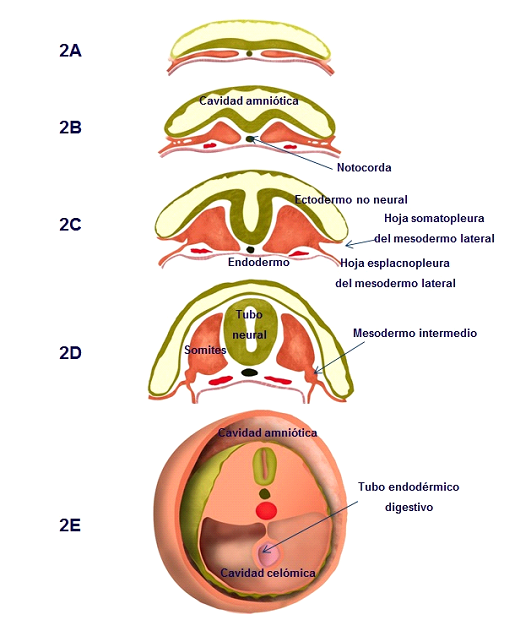
\includegraphics[width=0.4\columnwidth]{A.imagenes/ACV-ANATANIM-FormacionMesodermo.png}}
    \subfigure[Neurulación o fases de formación del tubo neural.]{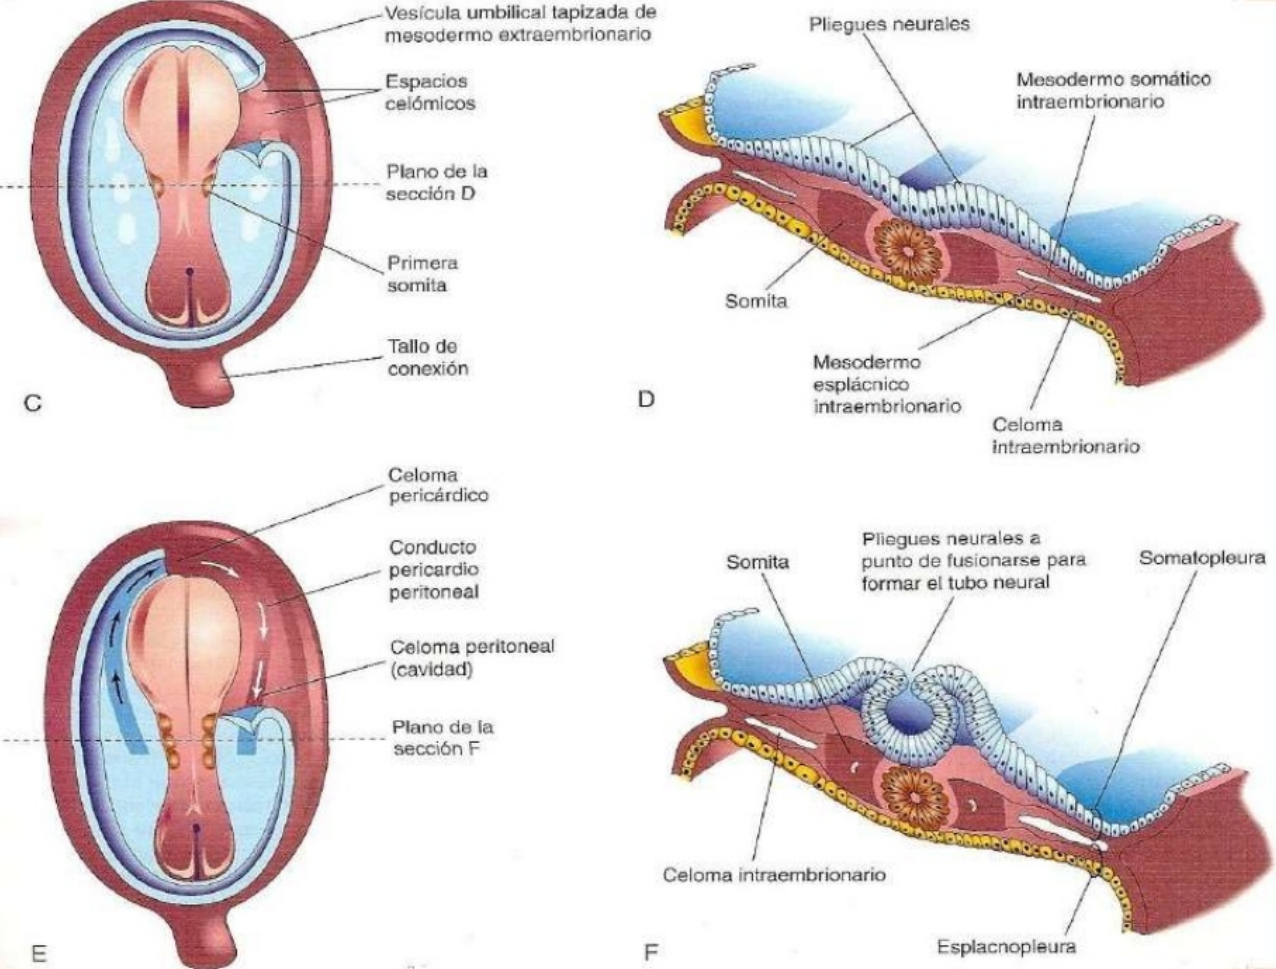
\includegraphics[width=0.59\columnwidth]{A.imagenes/ACV-ANATANIM-DiferenciacionNeurodermo.png}}
    \caption[Diferenciación del mesodermo]{Diferenciación del mesodermo.}
\end{figure}



